\chapter{Methodology}
In this chapter we will explore the approaches followed to plan, organise, manage and develop the project. We will discuss the methodologies that were adapted and combined to complete the research and development of the project along with why they were implemented. This section aims to give insight to the reader how the project transformed from research to final software while collaborating as a team.

Throughout our four years at GMIT a major emphasis was always placed on the importance of software development methodologies and the importance of choosing the most suitable methodology for a given project. There are numerous  methodologies that have all been extensively explored such as Waterfall, RAD (Rapid Application Development) and Extreme Programming to name a few. For this project we chose the main modern leader also based on the methodologies used by our employers, an approach known as Agile programming.

% ========================== Version Control  ========================== 
\section{Version Control}
In regards to version control with a focus on collaboration we decided to use the online Github Source Control Software. Github is a development platform allowing users to host and review code while also functioning as a simple yet powerful project management tool. Allowing the team to collaborate and support every aspect of the project management in one place it was an easy decision. 

Github enabled us to set up a team organisation that could store both our dissertation and our applied project repository's. We took full advantage of the many features that Github has to offer. The main function of Github allowed us to commit our work to the repositories and merge changes into the existing project. Another effective feature of Github is the project section, which is used to optimize project management. With a built in Kanban board we were able to track our progress while also logging any bugs or issues that arise \textit{(more details on this are given in Section \ref{KanbanSection})}. In respect to Software Development another impressive feature of Github is the ability to create branches. Essentially a branch is a pointer to a unique set of modifications to the original "Master" branch and is given its own branch name. Creating separate branches allows us to work on features and experiment with different functions without having an effect on the main project. When each feature is tested and complete, Github simple allows us to \textit{merge} our new changes back into the main \textit{master} branch.

% ========================== Development approach  ========================== 
\section{Agile development approach}
Agile Software Development is a concept that allows a product be delivered to the customer in incremental releases while also being highly flexible, allowing requirements to change and the scope of the project to increase without major consequences on the design or current task\cite{agile}.

We chose Agile as it stood out and had many benefits to our own project:
(https://project-management.com/10-key-principles-of-agile-software-development/=======imagelink for ref)

\begin{figure}[H]
\begin{minipage}{.5\textwidth}  %listing bloc will have 50% of the line width 
\lstset{linewidth = 4cm, breaklines=true} %set your listing lines widths, and set breaklines to true
\begin{itemize}
\item Develop small, incremental releases
\item Active user involvement
\item Evolving requirements
\item High level requirements
\end{itemize}

\end{minipage}
\qquad %space between listing bloc and the figure
\begin{minipage}{0.4\textwidth} %figure will have the remaning 40% of the line width
\includegraphics[scale=.4]{img/agile.jpg} %the image must be resized or scaled if needed
\caption{The Agile Cycle}
\end{minipage}
\end{figure}

Firstly as we were exploring all new languages, frameworks and libraries Agile allowed us to easily continuously integrate new features as our knowledge portfolio grew. Another major advantage was that this approach allowed us to have a working model every week rather than releasing the project in one release as would be in the Waterfall methodology. This alone gave us the opportunity to review each weeks progress while also receive continuous feedback from our mentors.

From the outset of the planning phase the main requirements and features of the software were identified. Subsequently we broke these features down into sub tasks which enabled complex tasks to be completed with simplicity. In the following subsections we will explain how using two prominent features of Agile, namely Kanban and Sprints we could track our development and monitor our progress.


% ========================== KanBan  ========================== 
\subsection{KanBan} \label{KanbanSection}
The Kanban Method is a means to design, manage, and improve flow systems for knowledge work. The method also allows organizations to start with their existing workflow and drive evolutionary change. They can do this by visualizing their flow of work, limit work in progress and stop starting and start finishing \cite{kanban}.

The Kanban Method gets its name from the use of kanban - visual signaling mechanisms to control work in progress for intangible work products. In simplicity Kanban is based around a Kanban board featuring Kanban cards (sticky notes). Thus allowing the full team to visualize crucial project information such as what tasks need doing, what tasks are in progress (and by whom) and what tasks are complete. 

\begin{figure}[H]
  \includegraphics[width=\linewidth]{img/kanban.PNG}
  \caption{Github Kanban}
  \label{fig:kanban}
\end{figure}

Figure  ~\ref{fig:kanban} above contains a snapshot of the projects Kanban board during development using the online project utility available on Github. This allowed us, as a team, to see at any point in time, what tasks needing doing, which were in progress or completed, while also tracking bugs and and a section to propose improvements.

% ========================== Sprints   ========================== 
\subsection{Sprints}
The term Sprint is mainly used in the Scrum framework of the Agile methodology and for our project worked hand-in-hand with Kanban. A Sprint is a timed iteration of the continuous development cycle with a scrum being a meeting style discussion used to adapt feedback. During development our default sprint duration was one week starting directly after each weekly review with our supervisor and ending at the following review where we would conduct a sprint plan. The aim of the sprint plan is to as a team reach two key decisions, \textbf{Sprint goal} what can be achieved in the sprint and \textbf{Sprint Backlog} the tasks to be completed in order to achieve the goal. During each sprint plan we would we would analyze the Kanban and discuss the following topics:

\begin{enumerate}
  \item What did we complete in our preceding sprint?
  \item What issues did we face?
  \item Is anything preventing us from progressing with a feature?
  \item Do any features need improvement?
  \item What backlog items to be implemented in the next sprint?
  \item What backlog items can we implement in the next sprint?
\end{enumerate}







% ========================== Choice of tech  ========================== 
\section{Choice of tech }
tech used and why
 Selection criteria for algorithms, languages, platforms and technologies.
 
% ========================== Testing , pass fail metrics  ========================== 
\section{Testing , pass fail metrics} 
As defined briefly in Section \ref{metrics} \texttt{Metrics for success or failure} our conditions were mainly focused and evaluated by user interaction. With the intention of monitoring  success we decided on tests to evaluate each metric:

\begin{enumerate}
  \item \textit{A  concise,  yet  comprehensive  dissertation  which  can  be  understood  by
anyone  regardless  of  the  initial  knowledge  of  the  technologies  implemented.}
  \item \textit{ Simple, easy to use, functional web application}
  \item \textit{A social platform that actually develops an online community}
  \item \textit{Teamwork Collaboration}

\end{enumerate}



Check out the nice graphs in Figure \ref{tikz:graphs}, and the nice diagram in Figure \ref{tikz:mydiagram}.

\begin{figure}
  \centering
  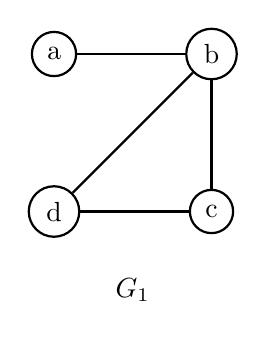
\begin{tikzpicture}
  \begin{scope}[every node/.style={circle,thick,draw}]
  \node (a) at (0,2) {a};
  \node (b) at (2,2) {b};
  \node (c) at (2,0) {c};
  \node (d) at (0,0) {d};
  \end{scope}
  \begin{scope}[every edge/.style={draw=black,thick}]
  \path (a) edge (b);
  \path (b) edge (c);
  \path (b) edge (d);
  \path (c) edge (d);
  \end{scope}
  \node () at (1,-1) {$G_1$};
  \end{tikzpicture}
  \hspace{1.5cm}
  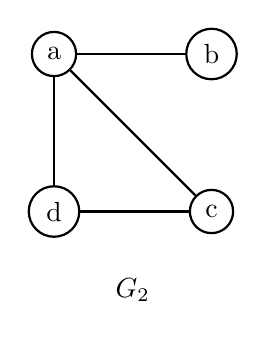
\begin{tikzpicture}
  \begin{scope}[every node/.style={circle,thick,draw}]
  \node (1) at (0,2) {a};
  \node (2) at (2,2) {b};
  \node (3) at (2,0) {c};
  \node (4) at (0,0) {d};
  \end{scope}
  \begin{scope}[every edge/.style={draw=black,thick}]
  \path (1) edge (2);
  \path (1) edge (3);
  \path (1) edge (4);
  \path (3) edge (4);
  \end{scope}
  \node () at (1,-1) {$G_2$};
  \end{tikzpicture}
  \caption{Nice pictures}
  \label{tikz:graphs}
\end{figure}


\begin{figure}
  \centering
  \begin{tikzpicture}[node distance=6cm]
  \node (a) [rect] {A Big Blue Block};
  \node (b) [oval, right of=a] {And His Oval Friend};
  \draw [line] (a) -- (b);
  \end{tikzpicture}
  \caption{Nice pictures}
  \label{tikz:graphs}
\end{figure}